\subsection{Inferring functional connectivity from simulated calcium imaging data} \label{sec:results:inference}

With neural population activity simulated as described in the previous section, we used our inference algorithms to reconstruct the functional connectivity matrix from simulated fluorescence data. Specifically, we estimated the connectivity matrix using both the embedded-chain-within-blockwise-Gibbs approach as well as factorized approximation. Figure \ref{fig:scatters} shows that factorized approximation was able to provide reconstructions almost as accurately as the exact embedded-chain-within-blockwise-Gibbs approach, $r^2=0.47$ versus $r^2=0.48$, when parameters corresponded to a realistic experiment, given $10$ minutes of simulation data, and a population of $N=25$ neurons. We also estimated the weights using the true spike trains, $r^2=0.7$ (not shown), and the spike trains down-sampled to the frame rates of calcium imaging, $r^2=0.57$. Importantly, the quality of our estimates using the fluorescence traces alone (and no electrophysiological data) approached that using the true down-sampled spike trains.  

%was worse than those obtained from the the true down-sampled spike trainsm although for SNR of fluorescence data the $r^2$ values for obtained reconstructions approached that of down-sampled true spike trains, Figure \ref{fig:recvar-SNR}. Example of what we understand by high SNR (can be used for functional connectivity inference) and low SNR (cannot be used for functional connectivity inference) are shown in Figure \ref{fig:recvar-SNR} on two fluorescence traces from real in-vivo data.
%
%Fluorescence data is generally acquired at low frame rate and, so, one of its main limitations is bad time-resolution of the observed spike trains. To determine the impact of this constraint on the connectivity reconstructions, and, thus, to determine how close calcium imaging may approach reconstructions from spike trains directly observed under comparable conditions, we conducted this experiment. We observed that at intermediate SNR reconstructions from calcium imaging closely resemble(0d such obtained directly from spike trains, and at higher SNR reconstruction with the quality same with original spike trains was achieved, Figure \ref{fig:scatters} and \ref{fig:recvar-SNR}.
%
%\begin{align}
% \label{eqn:likelihoodGLMmoda}
% &E[\ln P[n_i(t)| \bh(t); b_i, k_i, \bw_i, S^{ext}(t)]
% 	=\sum_t \left( n_i(t) \ln J_i(t) - (1-n_i(t)) \exp(J_i(t)) \Delta \right), \\
% \label{eqn:likelihoodGLMmodb}&J_i(t)=b_i+\sum\limits_j \sum\limits_{t'<t} \w_{ij}(t-t')n_{j}(t')=
% b_i+\sum\limits_j w_{ij} h_j(t).
% \end{align}
%
%The sum in Eqs.~\eqref{eqn:likelihoodGLMmoda} and \eqref{eqn:likelihoodGLMmodb} was over the sample of $\{n_i(t)\}_{i\leq N}$, produced with our spike sampling algorithm, discretized over the time-bins $t'$ with the width corresponding to the calcium imaging frame rate (i.e. 30 ms for 33 Hz and 15 ms for 66 Hz). In one of the two cases we considered, EPSP time-profiles were assumed to be ``known'' exponential, and the weights were estimated using reduced histories $h_{i}(t)=\sum_{t'<t} \exp(-(t-t')/\tau^h)n_{i}(t')$ with the time constant $\tau^h=10$ ms (i.e. second equation in Eq.~\eqref{eqn:likelihoodGLMmodb}). In the second case we considered, the time dependence of $\w_{ij}(t)$ was assumed to be unknown and the first equation in Eq.~\eqref{eqn:likelihoodGLMmodb}) was used to correlate $n_i(t)$ with $n_j(t')$ for $t'<t$ up to a given depth $m$.  In this latter case, since each next term in Eq.~\eqref{eqn:likelihoodGLMmodb}) was significantly smaller than the previous one, we found that the best results were obtained if we took $m=1$ (i.e. minimizing number of unknown variables given certain amount of data). In either case, we described the connection weight between two neurons by a scalar quantity $w_{ij}^s=\text{sign}(\w_{ij})\max_{t} |\w_{ij}(t)|$, which thereafter was used to compare true and reconstructed connectivity weights in all examples below.

\begin{figure}[h]
\centering
\begin{minipage}[c]{0.45\hsize}
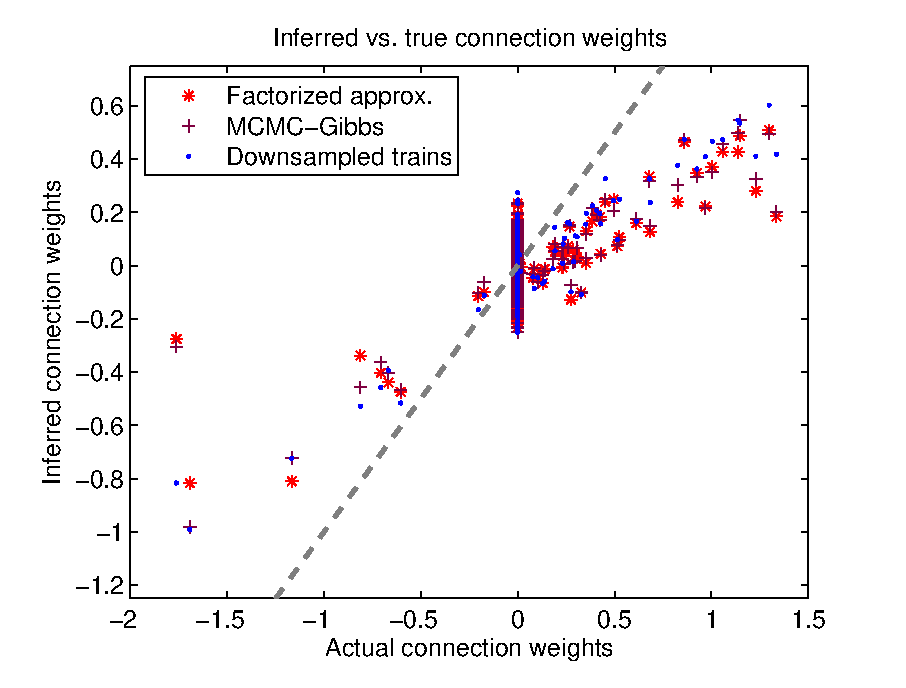
\includegraphics[width=\hsize]{../figs/FigureA3_scatter_three}
\end{minipage}
\begin{minipage}[c]{0.45\hsize}
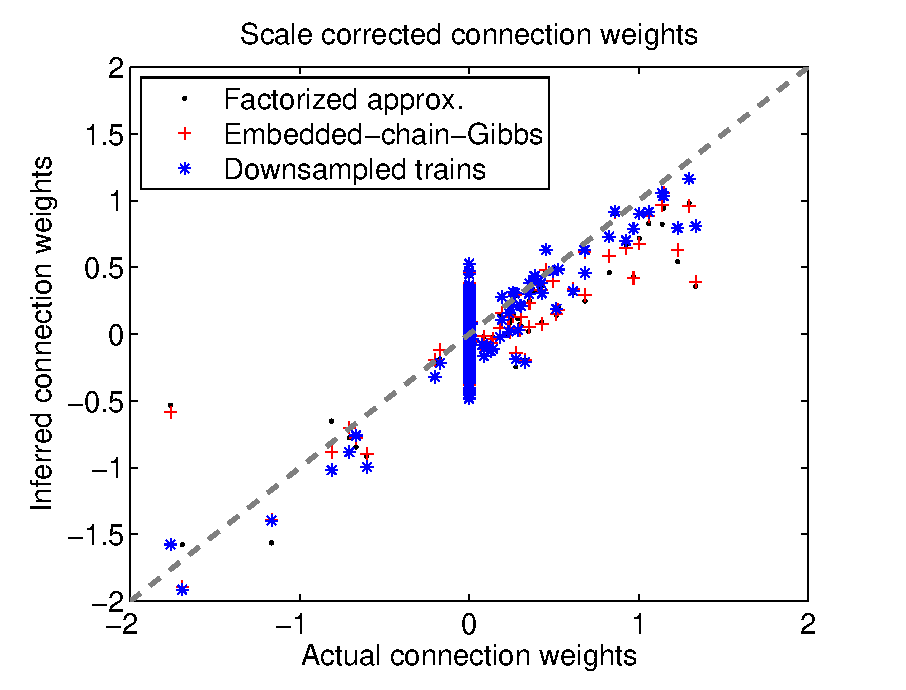
\includegraphics[width=\hsize]{../figs/FigureA3_scatter_three_corrected}
\end{minipage}
\caption{Functional connectivity matrix can be reconstructed from calcium imaging data. Inferred connection weights are shown in a scatter plot versus real connection weights, with inference performed using factorized approximation, exact embedded-chain-within-blockwise-Gibbs approach, and spike trains down-sampled to the frame rate of the calcium imaging. A network of $N=25$ neurons was used, firing at $\approx 5$ Hz, and imaged for 10 min at intermediate SNR (photon budget 10 Kph/neuron/frame; see below). The factorized approximation had an $r^2=0.47$, as compared with the embedded-chain-within-blockwise-Gibbs method's $r^2=0.48$, and $r^2=0.57$ for down-sampled spike trains. The inferred connectivity show a clear scale error (left panel), which we correct using our theoretical scale correction factor (right panel; see Section \ref{sec:scale} for details).} \label{fig:scatters} \end{figure}

\subsection{Impact of coarse time discretization of calcium imaging data and scale factor of inferred connection weights} \label{sec:scale}

As suggested by Figure \ref{fig:scatters}, upon inferring connection weights using down-sampled spike trains (or noisy versions thereof), a scale error is introduced. This is curious because our model was designed to be asymptotically unbiased \cite{PAN03d}. Possible causes of this scale error include (i) insufficient data,  (ii) model misspecification (the simulated model did not conform exactly to our assumed model, due to the shape of PSPs; see Methods for details), or (iii) coarse time discretization.  To investigate what extent of the scale error is caused by the coarse time discretization, we performed the following heuristic argument.

The sufficient statistic for estimating the weights to neuron $i$ in our model is simply $E[X_i(t), \bX (t-\Delta)| \bF; \bth]$, which depends only on $t$ and $t-\Delta$.  If, however, spike trains are down-sampled, such that observations are made only several time-bins, this statistic is not available.  More specifically, it becomes unclear whether certain presynaptic spikes occurred in $t$ or $t-\Delta$.  Thus, some fraction of spikes causally involved in postsynpatic firing will appear coincidental.  The faction of spike that appear coincidental, but are actually causal, corresponds to the expected scale error.

To formalize the above argument, consider the following significantly simplified case of two neurons coupled with a small weight $w_{ij}$, simulated with a time step size of $\Delta$. The sufficient statistic for estimating $w_{ij}$ is simply the expected value of a spike from neuron $i$ at time $t$, given a spike from neuron $j$ at $t-\Delta$:
\begin{align} %\label{eqn:scale:leadin-1}
SS&=E\left[n_i(t) | n_j(t-\Delta)=1\right] %\nonumber \\
=E\left[1-\exp\left(-\text{e}^{b_i+w_{ij}h_{ij}(t)}\right)\right]  \nonumber \\
&\approx \exp(-b_i) \Delta + f'(b_i) \exp(-t/\tau_h) %\nonumber \\
\approx  \exp(-b_i) \Delta + f'(b_i) w_{ij}\tau_h, \label{eqn:SS}
\end{align}
where $f'(b)=df/dXXX$, and $b_i \gg w_{ij}$. The above approximations follow due to XXX, and are required because the expected value is analytically intractable due to the $h_{ij}(t)$ term. 
% where 
% \begin{align}
% \tilde{h}_{ij}^k(t)=\left((1-\Delta \tau^h)h_{ij}(t-\Delta)+1\right)^k
% \end{align}

Now, if the spike trains were down-sampled by a factor $d$, we must further approximate the sufficient statistics. In particular, we would not know precisely in which time of $d$ time-bins the spike from neuron $j$ occurred.  Thus, the best we could do would be:
\begin{align} %\label{eqn:scale:leadin-1}
SS_d=&\sum_{k=1}^{d} E\left[n_i(t) | n_j(t-k\Delta)=1, \{n_j(t-k'\Delta)\}_{k' \neq k}=0\right] %\nonumber \\ &
=\sum_{k=1}^d E\left[1-\exp\left(-\text{e}^{b_i+w_{ij}\tilde{h}_{ij}^k(t)}\right) \right] \nonumber \\
&\approx \exp(-b_i) d\Delta + f'(b) \int\limits_0^\Delta \frac{\text{dt}'}{\Delta} \int\limits_{\Delta}^{\Delta + \mathcal{T}} \text{dt} w_{ij}\exp(-(t-t')/\tau^h) \nonumber \\&
\approx \exp(-b_i) d\Delta +  f'(b)w_{ij}\frac{1-\exp(-\Delta/\tau_h)}{\Delta/\tau_h^2}, \label{eqn:SS_d}
\end{align}
\noindent where $\tilde{h}_{ij}^k(t)$ is the expectation of $h_{ij}(t)$ given a spike from neuron $j$ at $k$ time-bins ago, the approximation follows using the same reasoning as above. The scale error that we expect to obtain from this coarse time discretization is thus: 

\begin{align} \label{eqn:bias}
	\tilde w_{ij} \approx w_{ij} \times\text{scale factor} = w_{ij}  \frac{SS}{SS_d} = w_{ij} \frac{1-\exp(-\Delta/\tau_h)}{\Delta/\tau^h}.
\end{align}

% Unfortunately, we cannot evaluate either $SS$ or $SS_d$ exactly, due to the exponential in $\tilde{h}_{ij}^k(t)$.  Assuming that $\tau^h \ll K \ll 1/r$, we can, however, approximate both by XXX:
% \begin{align}
% 	% SS \approx & r \mathcal{T} + f'(b) \sum_{k=1}^K w_{ij} \exp(-t/\tau^h) \nonumber \\
% 	% 	\approx & r \mathcal{T} + f'(b) w_{ij}\tau^h, \label{eqn:SS}\\
% 	SS_d  	\approx& r \mathcal{T} + f'(b) \int\limits_0^\Delta \frac{\text{dt}'}{\Delta} \int\limits_{\Delta}^{\Delta + \mathcal{T}} \text{dt} w_{ij}\exp(-(t-t')/\tau^h) \nonumber \\
% 		\approx & r \mathcal{T} +  f'(b)w_{ij}\frac{1-\exp(-\Delta/\tau^h)}{\Delta/(\tau^h)^2}. \label{eqn:SS_d}
% \end{align}
% Solving for $w_{ij}$ in terms of $SS$ and $SS_d$, and plugging the resulting values into Eq.~\ref{eqn:scale} yields:
% \begin{equation}\label{eqn:bias}
% w_{ij}\approx \frac{1-\exp(-\Delta/\tau^h)}{\Delta/\tau^h} w_{ij}.
% \end{equation}

% \begin{equation}
% E[n_i(t), n_j(t+\Delta_s) | F_i,F_j] \approx E[n_i(t), n_j(t+\Delta_o) | F_i,F_j]
% \end{equation}
% Our task here is to evaluate the scale error introduced by this approximation, and derive an analytical correction factor.  Let ``causal'' spike-pairs indicate spike-pairs when neuron $j$ spikes in a time bin \emph{preceding} the spike in neuron $i$.  Similarly, Let ``coincident'' spike-pairs indicate those spike-pairs for which both neurons spike within the same time bin.  The coarse time discretization implies that some fraction of causal spike-pairs will appear as coincident spike-pairs.  Thus, we anticipate that the scale error, $\xi$, will be proportional to:
% \begin{equation}
% \xi = \frac{E[\text{number of causal spike-pairs appearing as coincident spike-pairs}]}{E[\text{total number of causal spike-pairs}]}
% \end{equation}
% %Let $n_{ij}$ correspond to the total number of spike-pairs.  
% From Eq.~\eqref{eqn:glm:definition}, we have the probability of a spike from neuron $i$ in time bin $t$, given a spike from neuron $j$ in some previous time bin, $\mathcal{T}$:
% \begin{align}
% E[n_i(t) | n_j(t-\mathcal{T})] 
% &\approx 1-\exp(-\text{e}^{b + w_{ij} E[h_{ij}(t) | n_j(t-\mathcal{T})=1]} \Delta) 
% \end{align}
% where we define the expected spike history input conditioned on a spike from neuron $j$ at time $\mathcal{T}$:
% \begin{align}
% E[h_{ij}(t) | n_j(t-\mathcal{T})] &= \left((1-\Delta_s/\tau^h) E[h_{ij}(t-\Delta_s)] + 1\right)^{\mathcal{T}/\Delta_s}
% % = \sum_t n_i(t) P[n_i(t) | n_j(t-\mathcal{T})]  
% % = \sum_t  1-\exp(-\text{e}^{b + w_{ij} h_{ij}(t)} \Delta)
% %\exp{-t/\tau^h}
% %\approx r \mathcal{T} + f'(b) \int^{\mathcal{T}}_0  w_{ij} \exp(-t/
% %\tau^h) dt = XXX
% \end{align} 
% When we use a coarse time discretization, Eq.~\eqref{eqn:E[h]} changes by replacing each $\Delta_s$ by a $\Delta_o$.  
% 
% this above expectation changes to:
% \begin{align}
% E[h_{ij}(t) | n_j(t-\mathcal{T})] &= \left((1-\Delta_o/\tau^h) E[h_{ij}(t-\Delta_s)] + 1\right)^{\mathcal{T}/\Delta_s}
% \end{align} 
% 
% Similarly, we can compute the number of causal spike-pairs that appear as coincident spike-pairs, given our coarse time discretization:
% 
% % In order to estimate $w_{ij}$, therefore, we need to empirically observe the number of spike-pairs such that the first neuron fired after the second neuron over some small period of time $\tau^h \ll \mathcal{T} \ll 1/r$. 
% % 
% % With this count, we empirically estimate the spike-triggered spiking probability of the first neuron, conditioned on the firing of the second neuron, and subsequently estimate the connection weight $w_{ij}$. Per time period $\mathcal{T}\ll 1/r$, the average number of such spike-pairs corresponding to connection weight $w_{ij}$ is:
% % \begin{equation}\label{eqn:scale:leadin-1}
% % n_{12} \approx r \mathcal{T} + f'(b) \int^{\mathcal{T}}  w_{ij} \exp(-t/\tau^h) dt.
% % \end{equation}
% % 
% % Now, assume that observed spike trains were additionally down-sampled into time-bins of size $\Delta$. We now only count the spike-pairs such that the spike of the first neuron and the second neuron occurred in different time-bins of size $\Delta$. Per time period $\mathcal{T}$, the average number of such spike-pairs in down-sampled spike trains can be calculated as follows. We consider all spike-pairs such that the spike of the second neuron occurred in one time bin, $t'\in [0,\Delta]$, and the spike of the first neuron occurred in any of the strictly subsequent time bins up to $\mathcal{T}$, $t\in [\Delta,\mathcal{T}]$. Taking into account that position of the first spike, $t'$, is uniformly distributed in $[0,\Delta]$, the average number of such spikes of the first neuron per spike of the second neuron, observed empirically, is:
% \begin{equation}\label{eqn:scale:leadin-2}
% n^{\Delta_o}_{12} \approx r \mathcal{T} + f'(b) \int\limits_0^\Delta \frac{\text{dt}'}{\Delta} \int\limits_{\Delta}^{\mathcal{T}} \text{dt} \exp(-(t-t')/\tau^h)
% = r \mathcal{T} +  f'(b)\frac{1-\exp(-\Delta/\tau^h)}{\Delta/{\tau^h}^2}.
% \end{equation}
% Plugging these results into Eq.~\eqref{eqn:bias_correction_factor}, we obtain:
% %\comment{If we were to naively apply GLM Eq.~\eqref{eqn:scale:leadin-1} in this latter case, we would have underestimated $w_{ij}$ by a factor $\approx (n^{\Delta_o}_{12}-r \mathcal{T})/ (n_{12}-r \mathcal{T})$, corresponding to smaller spike-triggered probability observed empirically in down-sampled spike-trains. This ratio is the scaling factor that we observe:}
% \begin{equation}\label{eqn:bias}
% \xi=\frac{n^{\Delta_o}_{12}-r \mathcal{T}}{n_{12}-r \mathcal{T}}\approx \frac{1-\exp(-\Delta/\tau^h)}{\Delta/\tau^h}.
% \end{equation}
% %\comment{In Figure \ref{fig:bias} we plotted Eq.~\eqref{eqn:bias} versus scale factor empirically observed from our simulations for different values of $\Delta$. As can be seen from}
% Figure \ref{fig:bias} shows that this theoretical approximation corresponds well to our empirically measured scale factor.

%% Spike trains, necessary to evaluate functional connectivity matrix $\bw$, here were inferred with discretization into time-bins corresponding to the frame-rate of calcium imaging fluorescence data. In principle, one could use super-resolution feature of \cite{Vogelstein2009} to obtain spike trains with arbitrarily small time step $\Delta\rightarrow 0$. However, the problem in that case is that the spikes, inferred from fluorescence data, contain inaccuracy in their temporal position $\approx 1/$frame-rate,  due to the time-discretization of the underlying fluorescence trace.Thus, when we super-resolve spikes using \cite{Vogelstein2009}, the spike pairs such that a spike of neuron $i$ closely follows a spike of neuron $j$ can be often confused with such where a spike of neuron $j$ closely follows a spike of neuron $i$. It, therefore, becomes impossible to determine which neuron fired first, and which neuron was pre-synaptic or post-synaptic in given pair of neurons $i$, $j$. More specifically,
%%because we rely on empirically counting close spike pairs in a set of spike trains to estimate the spike-triggered probabilities for spikes of different pairs of neurons, $i$ and $j$, which then allow estimating $w_{ij}$, above disordering of close spike pairs results in dramatic noise component in our estimate for the functional connectivity matrix by not allowing to effectively distinguish $w_{ij}$ and $w_{ji}$.
%when using $\Delta \rightarrow 0$, we observed large errors in $\bw$, $var[\bw] \propto \bw + \bw^T$ - because of inaccuracies in temporal position of spikesinferred from calcium imaging it became impossible to reliably distinguish which neuron causally preceded which other neuron, and only a-causal connectivity matrix $(\bw + \bw^T)/2$ could be determined.

% To circumvent this problem, we (down-)sampled the time-axis in bins of size $\Delta=1/$frame-rate, and treated all spike pairs that occurred within the same time-bin as coincidental. This successfully counteracted the above problem and, additionally, allowed to perform calculations substantially faster by using larger $\Delta$. At the same time, this resulted in scale bias that all our inferred  connectivity matrices consistently exhibited, Figure \ref{fig:scatters}. This bias may be successfully understood and corrected from the following time-discretization argument. Specifically, estimating the magnitude of the connection weight $w_{ij}$ is based on empirically evaluating the spike-triggered probability of neuron $i$ to fire, conditioned on neuron $j$. Most significant change in the spiking probability of neuron $i$, conditioned on neuron $j$, occurs within $\tau^h \approx 10-20$ msec from a spike of neuron $j$. When spike trains are down-sampled into large time-bins, e.g. $\Delta = 30$ msec, a significant fraction of close spike pairs appears coincident and not causal, as both spikes from neuron $i$ and neuron $j$ within $\approx \tau^h$ from each other are often assigned to the same time-bin. As we discussed in the previous paragraphs, such close spike pairs typically introduce a great deal of noise in the estimate of $\bw$. When $\Delta$ is large, however, most of such unreliable spike pairs would be considered coincidental and would not affect $\bw$ estimate. At the same time, all of such close pairs would be lost if we were to empirically evaluate the spike-triggered probabilities, which would have led us to believe in a lower than the actual  $w_{ij}$.
This is the scale bias that we observe. In Figure \ref{fig:bias} we plot the scale bias from Eq.~\ref{eqn:bias} versus that empirically deduced from our simulations for different values of $\Delta$. As can be seen in Figure \ref{fig:bias}, Eq. \ref{eqn:bias} describes observed scale bias very well.
	
An alternate way of dealing with this scale error would be to sub-sample spike trains, as discussed in \cite{Vogelstein2009}, to obtain spike train inferences at the desired temporal resolution.  This possibility was not pursued here, as this approximation was sufficient for this work.

\begin{figure}[h]
\centering
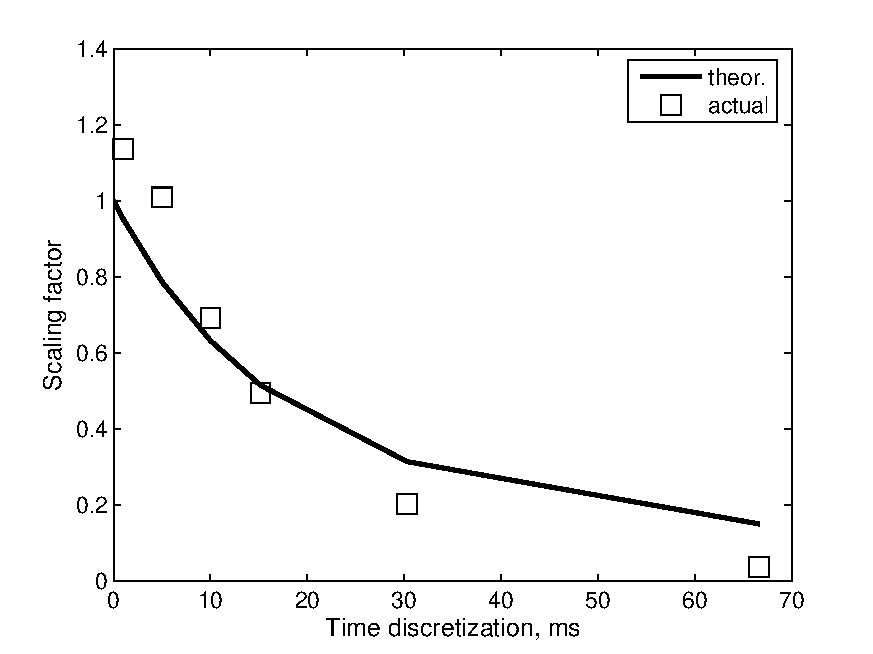
\includegraphics[width=3in]{../figs/FigureA4_scale_bias}
\caption{The low-frame rate of calcium imaging can explain the scale factor in inferred connectivity weights in Figure \ref{fig:scatters}.  Theoretically, scale factor may be evaluated by calculating what fraction of spikes from two neurons would occur within a single time-bin of width $\Delta$ (c.f. Eq.~\eqref{eqn:bias}).  
Plotted such theoretically calculated scale factor (line) vs. that observed empirically from our simulations (box), from a simulation of $N=25$ neurons, $T=10$ min. The error-bars correspond to 95\% confidence intervals for scale factor estimate.}
\label{fig:bias}
\end{figure}

\subsection{Impact of using priors on the inference}

Taking into account simple prior information about the connectivity matrix results in dramatic improvement of the inferred connectivity matrix using the same data.%; facilitating successful reconstruction from as little as $5$ min of calcium imaging data, and for $T\approx 10$ min achieving the same level of accuracy otherwise requiring up to $T\approx 1$ hour of calcium imaging, Figure \ref{fig:recvar-NT}. 
For example, imposing a sparse prior on a simulation of a network of $N=50$ neurons imaged for $T=10$ min, increased $r^2$ from $r^2=0.64$ to $r^2=0.85$ (Figure \ref{fig:sparse}). Furthermore, the weights estimated using the sparse prior more reliably provide true connectivities, as well as the appropriate sign (i.e., exicitatory or inhibitory) of each presynaptic neuron (Figure \ref{fig:distros}). Unfortunately, introducing a sparse prior further scales connectivity estimates, invaliding our analytic scale correction factor.  Thus, a sparse prior can provide a more rapid estimate of relative connection strengths, but not absolute connection strengths, at this time. 

Dale's prior, on the other hand, only leads to $\approx 10\%$ change in $r^2$ of the reconstructed connectivity matrix for this simulation, and was not found significant. Further, imposing Dale's prior when the sparse prior was initially enforced, typically resulted in no improvement to $\bw$ at all (not shown).  As the sparse prior result achieved reconstruction accuracy close to the down-sampled spike train limit, there was limited room for improvement using Dale's prior, and thus, it is not pursued further here.

\begin{figure}[h]
\centering
\begin{minipage}[c]{0.45\hsize}
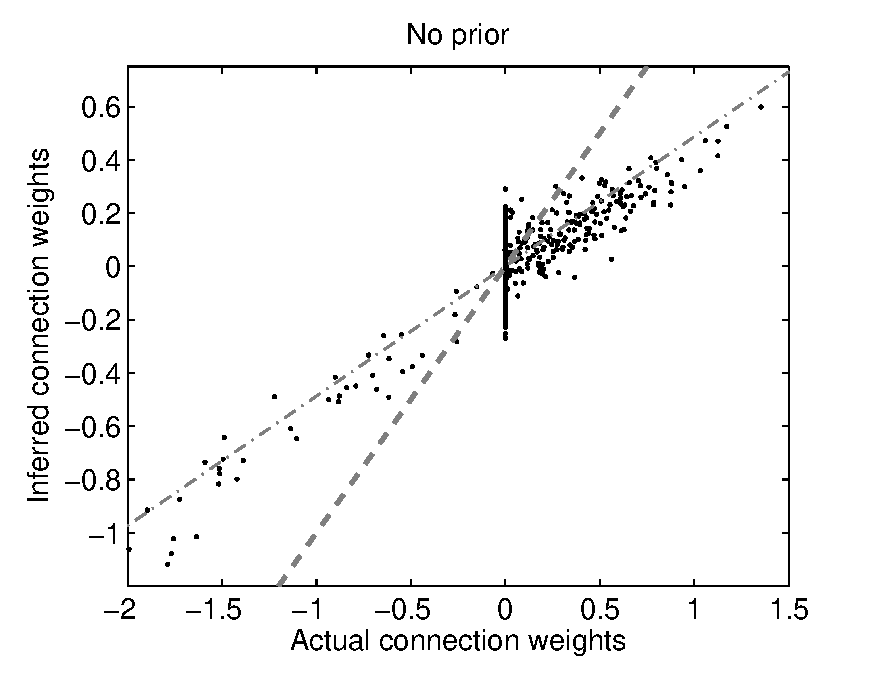
\includegraphics[width=\hsize]{../figs/FigureA10_regular_sol}
\end{minipage}
\begin{minipage}[c]{0.45\hsize}
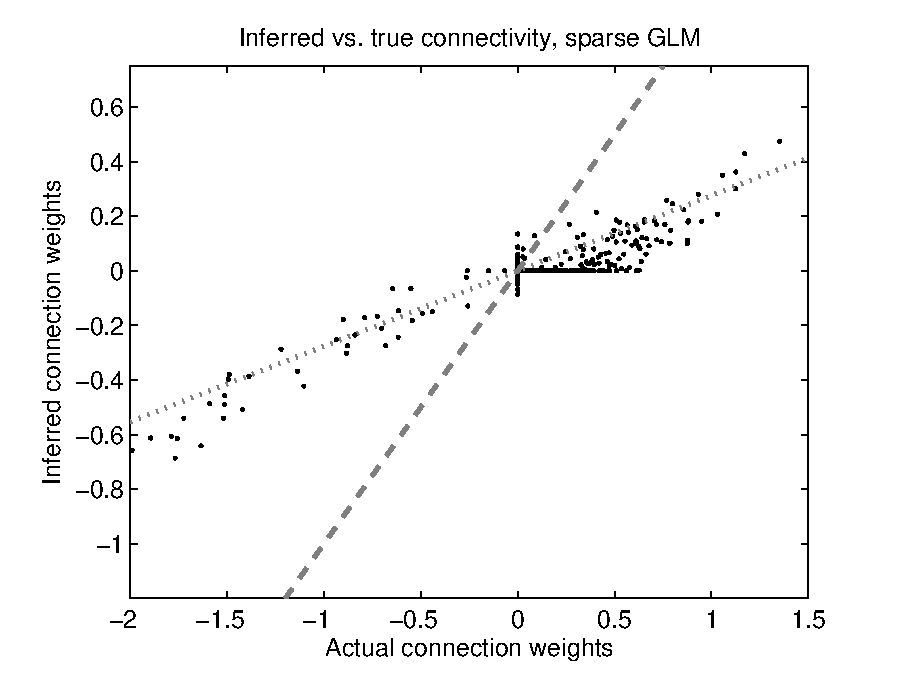
\includegraphics[width=\hsize]{../figs/FigureA10_sparse_sol}
\end{minipage}
\caption{Connection weights reconstructed using no prior ($r^2=0.64$; left panel) and a sparse prior ($r^2=0.85$; right panel) are shown in a scatter plot for a network of $N=50$ neurons, firing at $\approx 5$ Hz, and imaged for $T=10$ min. Clearly, the sparse prior reduces the relative error, as indicated by comparing the relative distance between the data points (black dots) to the best linear fit (black line), across the two panels.  }
\label{fig:sparse}
\end{figure}

\begin{figure}[h]
\centering
\begin{minipage}[c]{0.45\hsize}
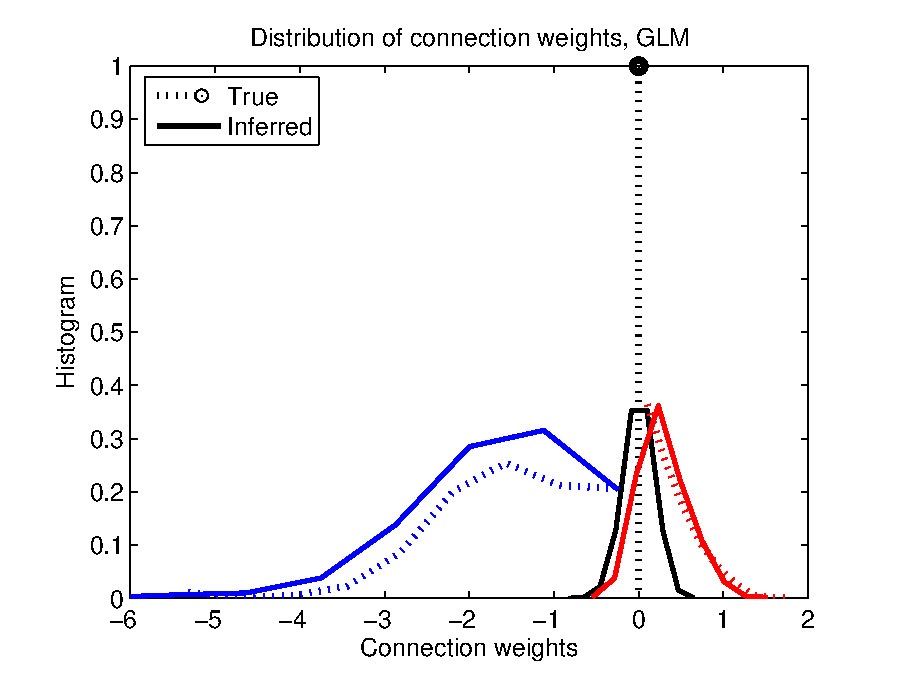
\includegraphics[width=\hsize]{../figs/FigureA3_hist_glm200}
\end{minipage}
\begin{minipage}[c]{0.45\hsize}
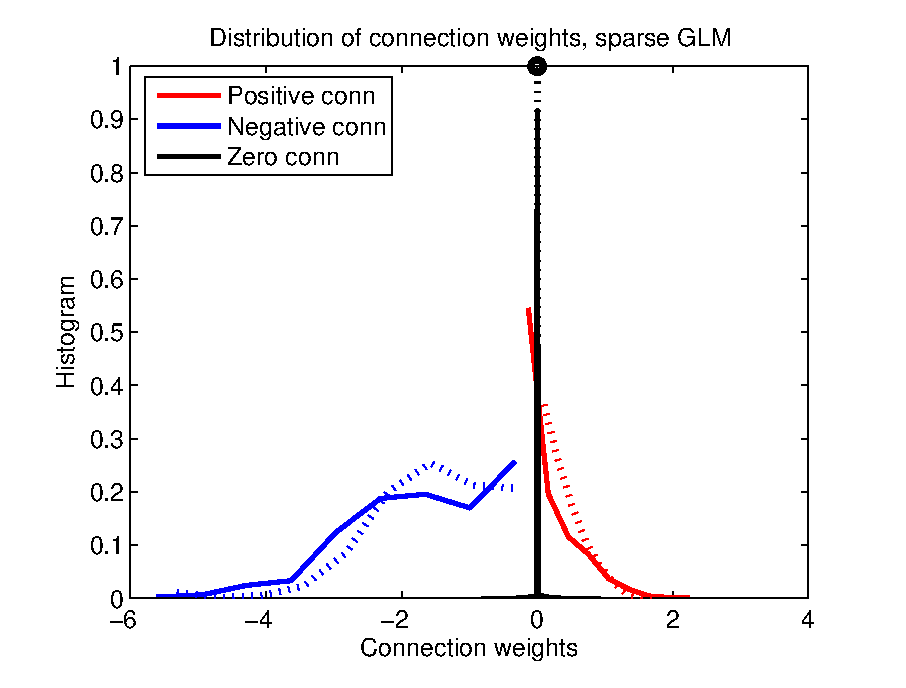
\includegraphics[width=\hsize]{../figs/FigureA3_hist_spa200}
\end{minipage}
\caption{Imposing a sparse prior on the distribution of connectivity weights, facilitates improving the inferred weights given the same amount of data. Shown here is the distribution of inferred connection weights using no prior (left panel) and a sparse prior (right panel) vs. true distributions. When the sparse prior is enforced, the appropriate number of connected pairs is identified (black lines), as well as the correct distribution of excitatory and inhibitory weights (red and blue lines, respectively). Distributions are shown for a network of $N=200$ neurons, firing at $\approx 5$ Hz, and imaged for $T=10$ min.}
\label{fig:distros}
\end{figure}


\subsection{Impact of experimental factors on estimator accuracy}

What minimal conditions for the experimental setup should be met to for sufficient reconstruction accuracy of the connectivity from calcium imaging data? In Figures \ref{fig:recvar}--\ref{fig:recvar-NT} we address this question. Figure \ref{fig:recvar} shows the quality of the inferred connectivity matrix as function of the imaging frame rate --- imaging frame rates $30$--$60$ Hz are needed to achieve meaningful reconstruction results. Frame rates $\approx 100$ Hz allow achieving the same level of the connectivity matrix reconstruction that is possible with the exact knowledge of the true spike trains. Imaging frame $30$--$60$ Hz are already in progress in existing experimental setups \cite{NguyenParker01,ReddySaggau05,Iyer06,SalomeBourdieu06,ReddySaggau08}, each with the ability to significantly increase imaging rate, but costing a reduction in the number of observable neurons.

\begin{figure}[h]
\centering
\includegraphics[width=3in]{../figs/FigureA5_recvar}
\caption{Accuracy of the inferred connectivity as function of the frame rate of calcium imaging.  A network of $N=25$ neurons, firing at $\approx 5$ Hz and imaged for $T=10$ min was simulated, and weights were inferred. At $100$ Hz, $r^2$ using calcium imaging data reached the same level of accuracy as using the true spike trains from this simulation, indicating the further improvement could not be achieved by a further increase in frame rate.}
\label{fig:recvar}
\end{figure}

Figure \ref{fig:recvar-SNR} shows the quality of the inferred connectivity matrix as function of effective SNR and photon budget. Operationally, we define effective SNR as
\begin{equation}
\text{eSNR}=\frac{E[F_i(t)-F_i(t-1)|n_i(t)=1]}{E[(F_i(t)-F_i(t-1))^2|n_i(t)=0]^{1/2}},
\end{equation}

\noindent and photon budget as $\gamma^{-1}$.  Photon budget corresponds to the number of photons collected from single neuron within a single frame, at the peak of fluorescence intensity. XXX i don't see how this is true. XXX Note that the relationship between photon budget and eSNR depends on a number of other parameters, $\{\alpha,\beta,\sigma^F, K_d\}$, as well as the calcium concentration (which depends on spike rate, as well as $\{\tau^c, A, C^b\}$). From our experience with the analysis of real cells \cite{Vogelstein2009}, the eSNR for data collected at $15$ Hz was $\approx 3$ for in vitro data sets, and $\approx 9$ for in vivo data sets (c.f. Figure \ref{fig:example_traces}). As can be seen from Figure \ref{fig:recvar-SNR}, the effective SNR necessary for optimal reconstructions given a particular frame rate was $\approx 5$. This eSNR corresponded to photon budgets of $\approx 10$ Kph/neuron/frame. Any lower, and reconstruction accuracy declined rapidly.  

\begin{figure}[h]
\centering
\begin{minipage}[c]{0.6\hsize}
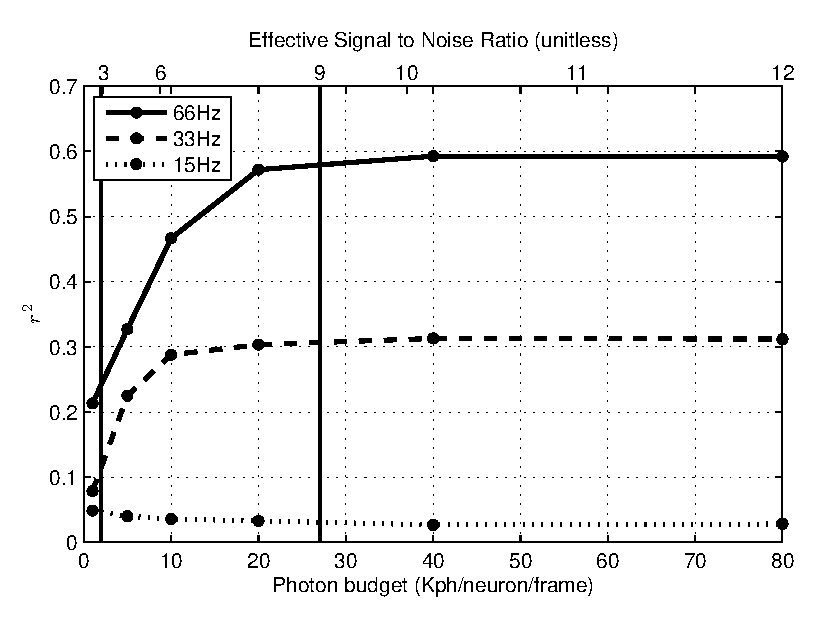
\includegraphics[width=\hsize]{../figs/FigureA6_recvar_SNRb}
\end{minipage}
\caption{Accuracy of inferred connectivity as function of the noise amount in the calcium imaging data, as quantified by (i) eSNR and (ii) thousands of photons, per frame, per neuron (Kph/frame/neuron), for frame rates of 1, 5, 10, 15, 33, and 66 Hz. Photon counts on the order of $10$--$20$ Kph/frame/neuron are required to achieve the upper bound determined by the frame rate. The connectivity matrix here was inferred from simulated fluorescence data using factorized approximation algorithm and the sparse prior. Simulation conditions are the same as in Figure \ref{fig:recvar}.  Vertical black lines correspond to the two example traces in Figure \ref{fig:example_traces}.}
\label{fig:recvar-SNR}
\end{figure}

Finally, Figure \ref{fig:recvar-NT} shows the quality of the inferred connectivity matrix as function of the experiment duration. The minimal amount of data for a particular $r^2$ depended substantially on whether the sparse prior was enforced. In particular, when not imposing a sparse prior, the calcium imaging duration necessary to achieve $r^2=0.5$ for the reconstructed connectivity matrix was $T\approx 10$ min, and $r^2=0.75$ was achieved at $T\approx 30$ min. With a sparse prior, $r^2>0.7$ was achieved already at $T\approx 5$ min. Furthermore, we observed that the accuracy of the reconstruction did not deteriorate with the size of the imaged neural population: the same reconstruction quality was observed with the same amount of data for $N=50$--$200$ neurons.  This, at first unexpected result, is the direct consequence of the structure of the covariance matrix for $\bw$, as will be discussed below. In all cases, good reconstructions were possible with only $T\sim 5$--$30$ min of calcium imaging data.

\begin{figure}[h]
\centering
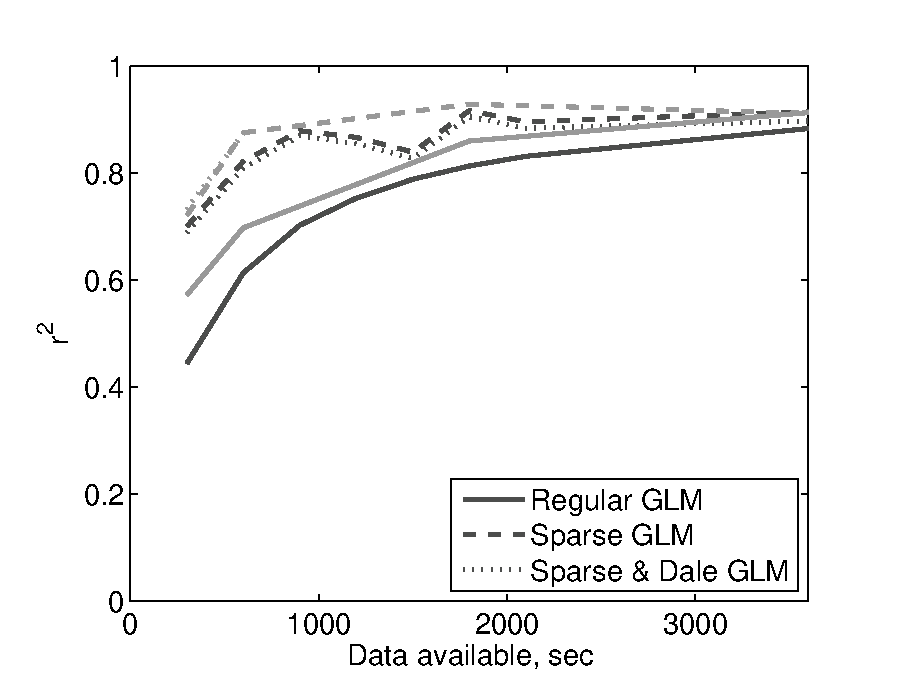
\includegraphics[width=3in]{../figs/FigureA7_recvar_NT}
\caption{Accuracy of inferred connectivity as function of the imaging time and neural population size. Incorporating a sparse prior dramatically increases the reconstruction's quality (dashed lines), over the no prior assumption (solid lines), given the same experimental duration. When the sparse prior is imposed, $T=5$ min is already sufficient to recover $70\%$ of the variance in the connection weights. Incorporating Dale's prior leads to only marginal improvement (dotted line). Furthermore, reconstruction accuracy does not depend on the neural population size, $N$. Here, neural population from $N=10$ to $N=200$ were simulated for different $T$, $N=100$ and $200$ are shown (black and gray, respectively).  Inhibitory weights for networks of different sizes were chosen to ensure mean firing rate $\approx 5$ Hz, although actual firing rate varied somewhat.}
\label{fig:recvar-NT}
\end{figure}

\subsection{Accuracy of the estimates and Fisher information matrix} \label{sec:methods:accuracy_Fisher}

Here we calculate theoretically the amount of spike trains data necessary to accurately estimate the functional connectivity matrix, $\bw$. For clarity, we assume here that $\Delta \rightarrow 0$, and so $f(J)\approx e^J\Delta$, and that the spike trains are known perfectly, i.e. there is no corruption due to inference from low-SNR calcium imaging data (an assumption validated by the above results). We also assume that the spikes only couple over a single time bin, so $h_{ij}(t)\equiv n_j(t-\Delta)$. Then, we can write the likelihood for the weights:
\begin{align}\label{eqn:fisher-glm}
% \begin{array}{rl}
-\ln P[\bw | \bX] &\propto -\ln P[\bX | \bw] =
\sum\limits_{i,t} \left[ n_i(t) \ln f(J_i(t)) + (1-n_i(t)) (1-f(J_i(t))) \right], \\
J_i(t) &= b_i(t) + \sum\limits_j w_{ij} h_{ij}(t) = b_i(t) + \sum\limits_j w_{ij} n_j(t-\Delta) 
%h_{ij}(t) &= n_j(t-\Delta)
.
% \end{array}
\end{align}
The Fisher information matrix for $P[\bw | \bX]$ is therefore:
\begin{multline}\label{eqn:fisher-def}
% \begin{array}{rl}
COV^{-1}_{ij;i'j'}=\left[\frac{\partial (-\ln P[\bw | \bX])}{\partial \w_{ij}\partial \w_{i'j'}}\right]
=\\-\delta_{ii'}\sum\limits_t\left[
n_i(t)n_{j}(t-\Delta)n_{j'}(t-\Delta)\left(-\frac{f'(J_i(t))^2}{f(J_i(t))^2} +
\frac{f''(J_i(t))}{f(J_i(t))}\right) -(1-n_i(t))n_{j}(t-\Delta)n_{j'}(t-\Delta)f''(J_i(t))\right],
% \end{array}
\end{multline}
where $f'$ and $f''$ correspond to the first and the second derivatives of our linking function (c.f Eq.~\eqref{eqn:glm:definition}), and $\delta_{ii'}$ is the Kronecker's delta symbol, i.e., $\delta_{ii'}=1$ for $i=i'$, and $\delta_{ii'}=0$ otherwise.  Letting $f(J)=e^J\Delta$, the first term in the sum in Eq.~\eqref{eqn:fisher-def} cancels out, and the rest may be rewritten as:
\begin{align}\label{eqn:fisher}
% \begin{array}{rl}
COV^{-1}_{ij;i'j'}
&=\delta_{ii'} T P[n_i(t)=0, n_j(t-\Delta)=1, n_{j'}(t-\Delta)=1]% \times \\&
\times E[e^{J_i(t)}|n_i(t)=0, n_j(t-\Delta)=1, n_{j'}(t-\Delta)=1] \nonumber \\
&= \delta_{ii'}T\left[(r \tau^h)\delta_{jj'}+O((r \tau^h)^2)\right]r.
% \end{array}
\end{align}
Here, $TP[n_i(t)=0, n_j(t-\Delta)=1, n_{j'}(t-\Delta)=1]$ describes the number of nonzero
terms in Eq.~\eqref{eqn:fisher-def}, corresponding to the condition that
$(1-n_i(t))n_{j}(t-\Delta)n_{j'}(t-\Delta)$ is only nonzero when 
$n_i(t)=0$, $n_j(t-\Delta)=1$, and $n_{j'}(t-\Delta)=1$.  We let $r=E[e^{J_i(t)}|n_i(t)=0, n_j(t-\Delta)=1, n_{j'}(t-\Delta)=1]$  correspond to the average value of $f''(J_i(t))$, conditional on such nonzero events.  $r\tau_h \ll 1$ is the probability for a neuron to spike over the time-interval $\tau_h$.

The Fisher information matrix is block-diagonal, $COV^{-1}_{ij;i'j'} \propto \delta_{ii'}$, due to the structure of the log-likelihood $P[\bX | \bw]$ (it is a sum over $i$ of independent terms), Eq.~\eqref{eqn:fisher-glm}.From Eq.~\eqref{eqn:fisher}, we observe that Fisher information matrix is predominantly diagonal, because $COV^{-1}_{ij;i'j'} \propto \delta_{ii'}\delta_{jj'}$, and thus the covariance matrix, $COV$, can be computed trivially:
\begin{equation}
COV = (rT)^{-1} (r \tau^h I + O((r \tau_h)^2))^{-1} = (r^2 \tau_h T)^{-1} I + O((r \tau_h)^2),
\end{equation}
\noindent where $I$ is the Identity matrix of appropriate size.  For successful determination of the functional connectivity matrix $\bw$, $COV$ should be made smaller than the typical scale $\langle \bw^2\rangle$, so we require that:
\begin{equation}
T \approx (\langle \bw^2 \rangle r^2  \tau^h)^{-1}.
\end{equation}
For typical values of $\bw^2\approx 0.1$, $r\approx 5$ Hz and $ \tau_h \approx 10$ msec, this estimate provides $T$ of the order of hundreds of seconds. This theoretical estimate of the necessary amount of fluorescent data is in good agreement with our simulations.

Finally, because $COV^{-1}$ is diagonal, this scale of $COV$ does not depend on the number of neurons in the imaged neural population, $N$. Thus, the variance of the estimate $\bw$ does not degrade with the size of the imaged population, $N$, for the same amount of data, $T$.

\subsection{Impact of strong correlations and deviations from generative model on the inference}

``Anatomical'' connectivity was recovered in our experiments despite potential problems noted in the literature, e.g. such as common input from correlated neurons \cite{Nykamp05,NYK06}, or unobserved neurons \cite{Vidne08}. %This is primarily due to the particular form of the activity in our neural networks, whereas firing of neurons occurred independently, thus, allowing GLM explore the full range of possible input configurations and disentangle common inputs.
Estimation of the functional connectivity is fundamentally rooted in observing changes in the spike rate conditioned on the state of the other neurons. Intuitively, such estimation can be compared to observing changes in $f({\bf n}(t))\propto\exp(\sum_j \w_{ij}n_j(t))$ for different neural configurations ${\bf n}(t)$, i.e. estimating a vector ${\bf w}_i$ from a number of dot-products ${\bf w}_i\cdot {\bf n}(t)$. In order to properly estimate all components of ${\bf w}_i$ the set of available ${\bf n}(t)$ should be rich enough to span all $N$ dimensions of ${\bf w}_i$. In case of independent firing such condition is clearly satisfied.  Should this condition be violated, however, e.g. due to high correlation between spiking of few neurons, spike trains may not provide access to the true vector ${\bf w}_i$, and the connection weights inferred from such activity data may effectively ``aggregate'' true connection weights in arbitrary linear combinations.

We carried out a simulation of hypothetical ``strongly'' coupled neural network, where in addition to weak sparse connectivity we introduced sparse random strong connectivity component. In a sense, we allowed a fraction of neurons to couple strongly to the other neurons, thus, making them ``command'' neurons ``driving'' the activity of the rest of the population. The strength of strong connectivity component was chosen to dynamically build up the actual firing rate from the baseline rate of $r=\exp(b)\approx 1$ Hz to approximately $5$ Hz. Such a network showed patterns of activity very different from the weakly coupled networks inspected above (Figure \ref{fig:rasters}, top right). In particular, a large number of highly correlated events across many neurons were evident in this network. As expected, our algorithm was not able to identify the true connectivity matrix correctly in this scenario (Figure \ref{fig:rasters}, bottom right panel).  For ease of comparison, the left panels show a ``typical'' network (i.e., one lacking many strongly coupled neurons), and its associated connectivity inference.  Note that the observability of the strongly coupled neurons does not save our inference.

\begin{figure}[h]
\centering
\begin{minipage}[c]{0.45\hsize}
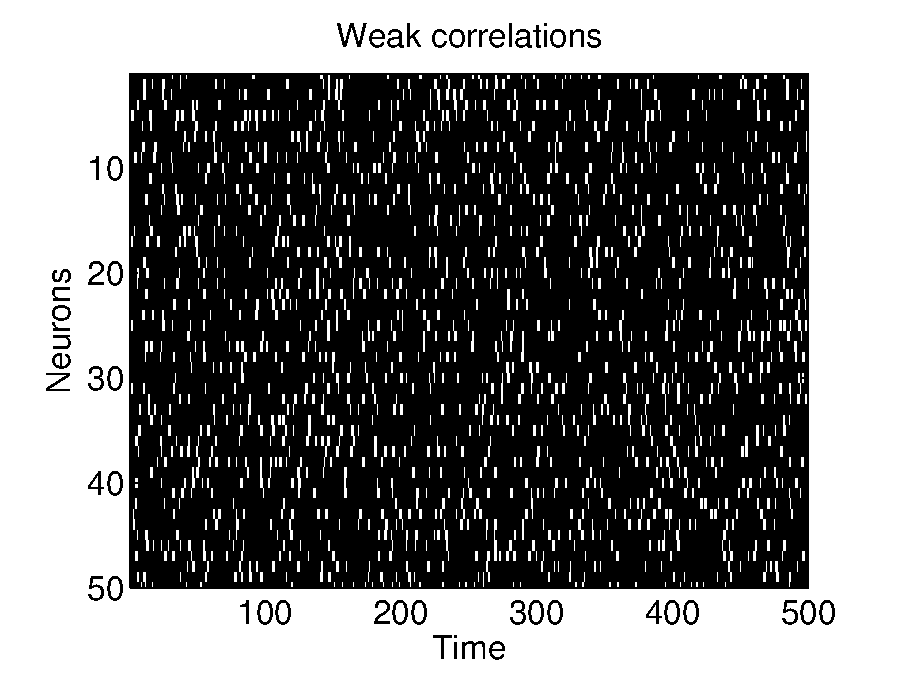
\includegraphics[width=\hsize]{../figs/Figure7b_raster_weak}
\end{minipage}
\begin{minipage}[c]{0.45\hsize}
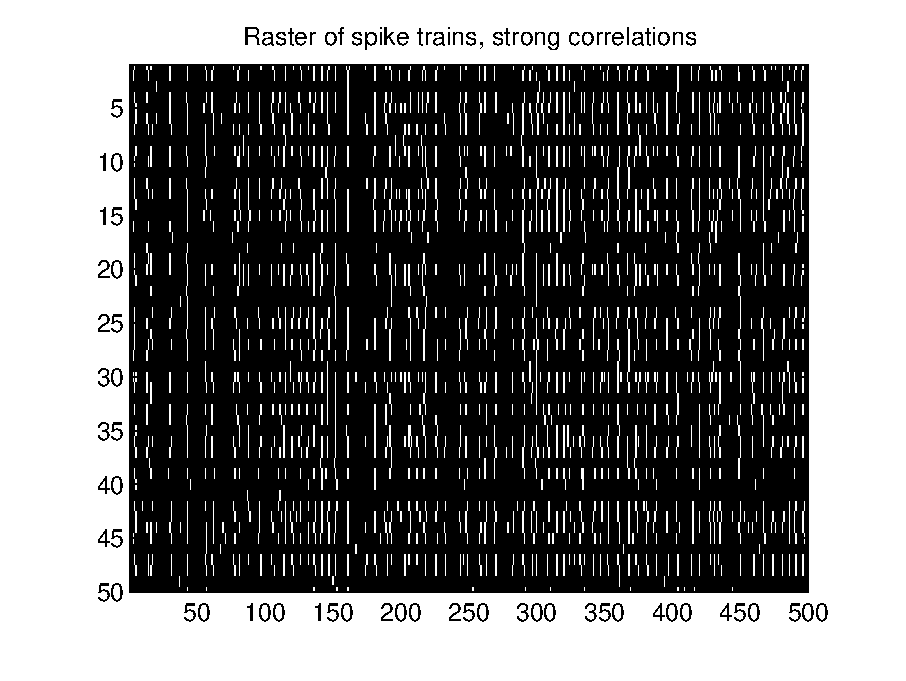
\includegraphics[width=\hsize]{../figs/Figure7a_raster_strong}
\end{minipage}
\begin{minipage}[c]{0.45\hsize}
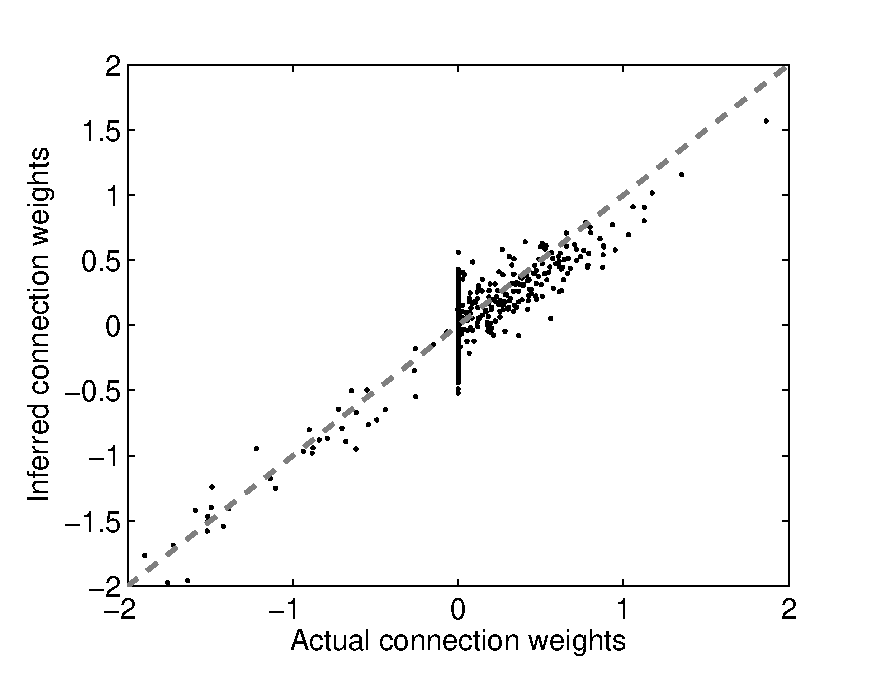
\includegraphics[width=\hsize]{../figs/FigureA8_weak_corr}
\end{minipage}
\begin{minipage}[c]{0.45\hsize}
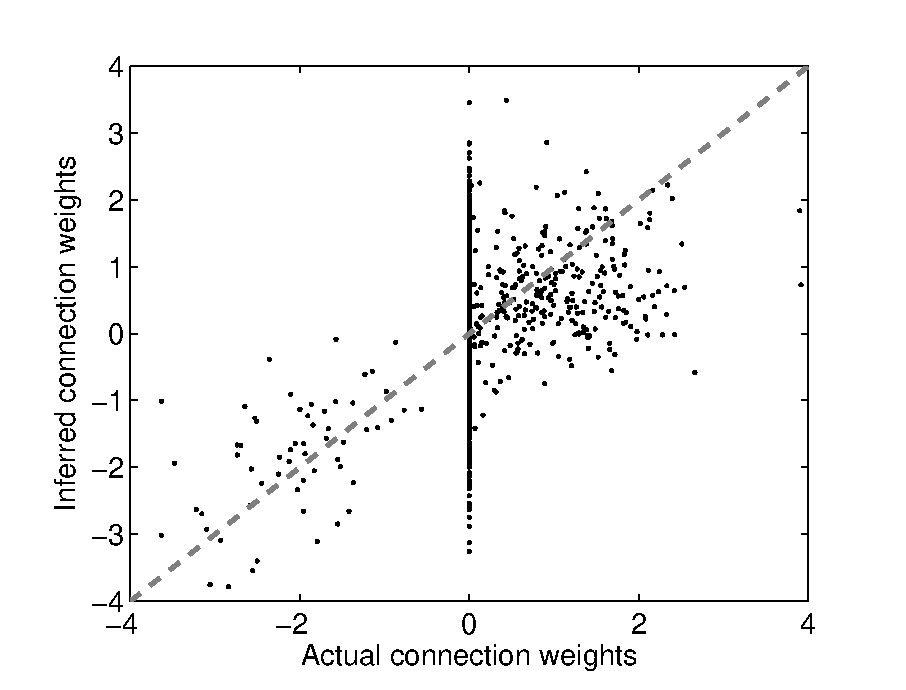
\includegraphics[width=\hsize]{../figs/FigureA8_strong_corr}
\end{minipage}
\caption{
Diverseness of observed neural activity patterns is required for functional connectivity to give access to the actual ``anatomical'' structure of the neural circuit. Here, 15 sec of simulated spike trains for a weakly coupled network (top left panel) and a network with strongly coupled component (top right panel) are shown. In weakly coupled networks, spikes are sufficiently uncorrelated to give access to enough different neural activity patterns to estimate the weights ${\bf w}$. In a strongly coupled case, many highly synchronous events are evident (top right panel), thus preventing observation of sufficiently rich ensemble of activity patterns. Accordingly, the connectivity estimates for the strongly coupled neural network (bottom right panel) does not represent the true connectivity of the circuit, even for the weakly coupled component. This is contrary to the weakly-coupled network (bottom left panel) where true connectivity is successfully obtained. Networks of $N=50$ neurons firing at $\approx 5$ Hz and imaged for $T=10$ min were used to produce this figure.}
\label{fig:rasters}
\end{figure}

On the other hand, our inference algorithm showed significant robustness to deviations of the actual data from our generative model. One important such deviation, which is likely to occur in the real experiments, is variation in the time scales of PSPs in different synapses. Up to now, all PSP time-scales were assumed to be the same in our inference algorithm as well as in the simulations, i.e., $\{\tau^h_{ij}\}_{i,j\leq N}=\tau_h$. In Figure \ref{fig:vartau} we introduce additional variability in $\tau_h$ from one neuron to another. Variability in $\tau_h$ results in added variance in the estimates of the connectivity weights $w_{ij}$ through $\tau_h$ dependence of the scaling factor Eq.~\eqref{eqn:bias}. Still, we found that such added variance was insignificant with $\tau_h$ varying for up to $25\%$ from neuron to neuron.

\begin{figure}[h]
\centering
\begin{minipage}[c]{0.45\hsize}
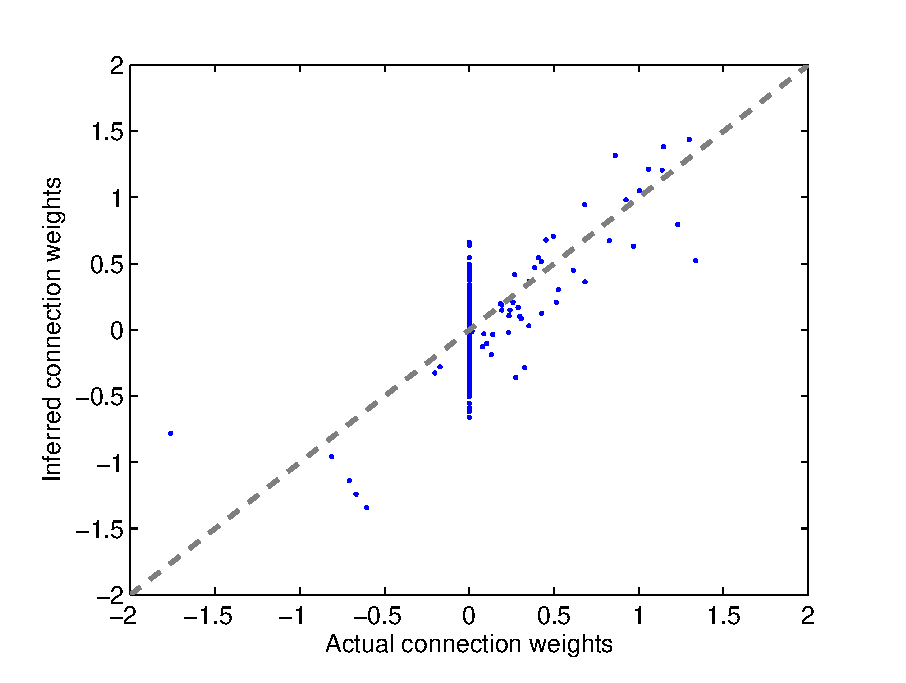
\includegraphics[width=\hsize]{../figs/FigureA9_all_same_sol}
\end{minipage}
\begin{minipage}[c]{0.45\hsize}
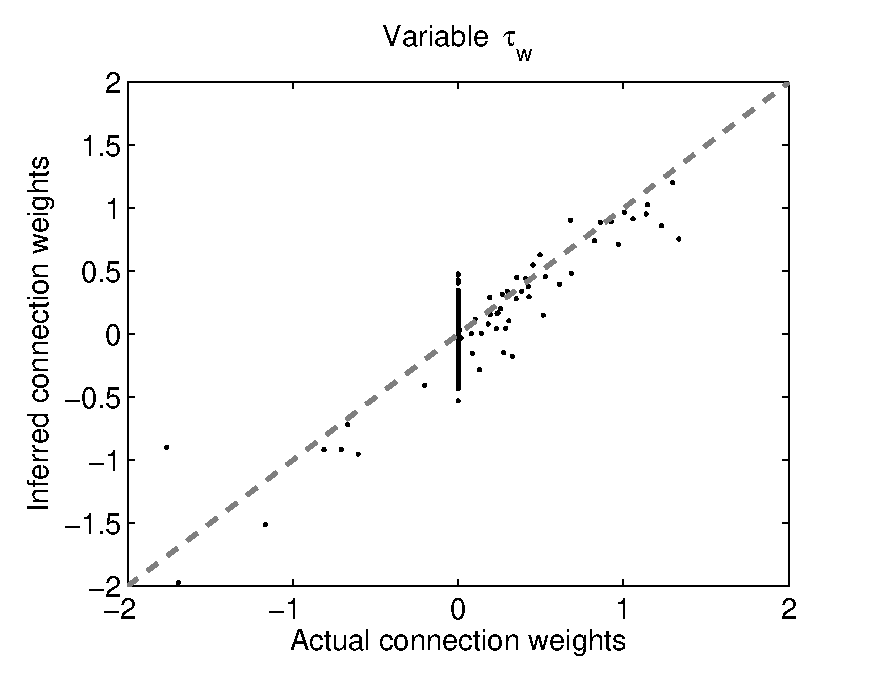
\includegraphics[width=\hsize]{../figs/FigureA9_variable_25}
\end{minipage}
\caption{
Inference is robust to deviations of the data from our generative model. One such deviation, that should be expected in real data, is variability in the PSP time courses from neuron to neuron, and possibly synapse to synapse. With up to $25\%$ variability allowed in PSP time scales $\tau_h$ (right panel), our algorithm provided reconstructions of almost the same quality as when all $\tau_h$'s were the same (left panel). Simulation conditions were the same as in Figure \ref{fig:recvar}.}
\label{fig:vartau}
\end{figure}

%Fig -: real data
% \begin{figure}[h]
% \centering
% \begin{minipage}[c]{0.45\hsize}
% 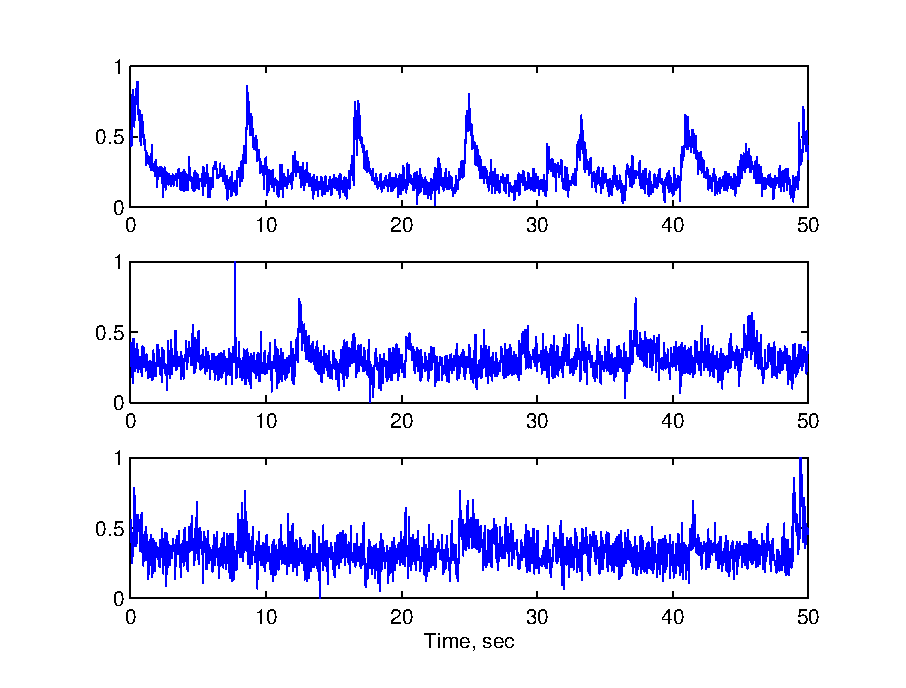
\includegraphics[width=\hsize]{../figs/FigureA11_real_traces}
% \end{minipage}
% \begin{minipage}[c]{0.45\hsize}
% 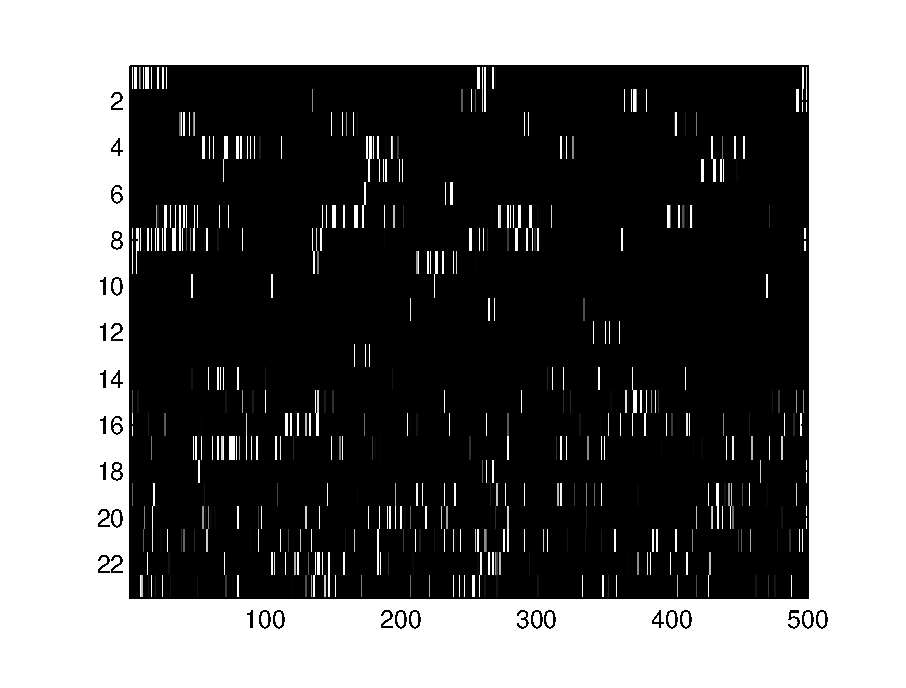
\includegraphics[width=\hsize]{../figs/FigureA11_real_raster}
% \end{minipage}
% \begin{minipage}[c]{0.3\hsize}
% 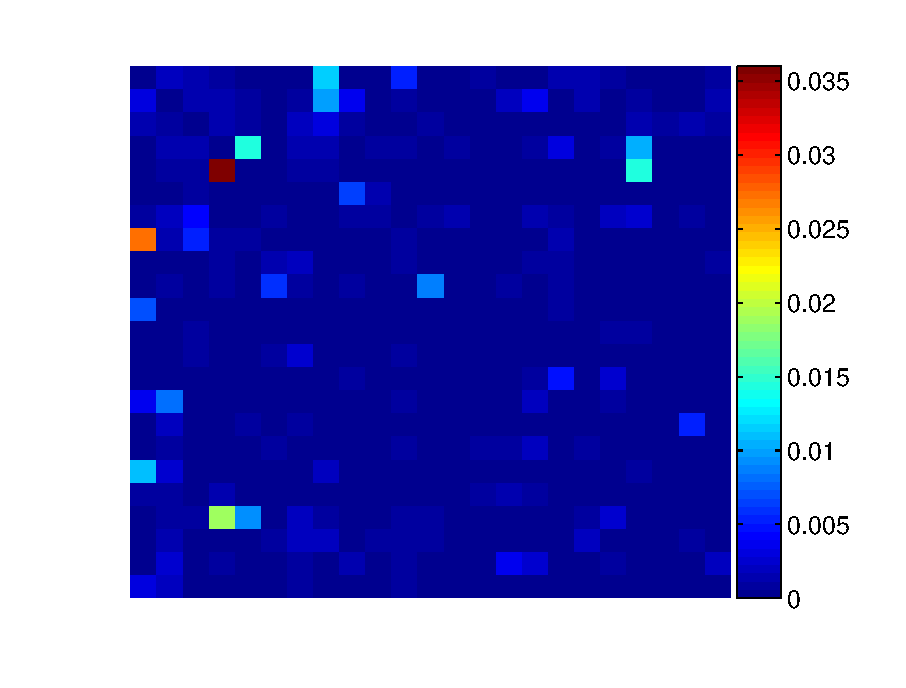
\includegraphics[width=\hsize]{../figs/FigureA11_real_Xcorr}
% \end{minipage}
% \begin{minipage}[c]{0.3\hsize}
% 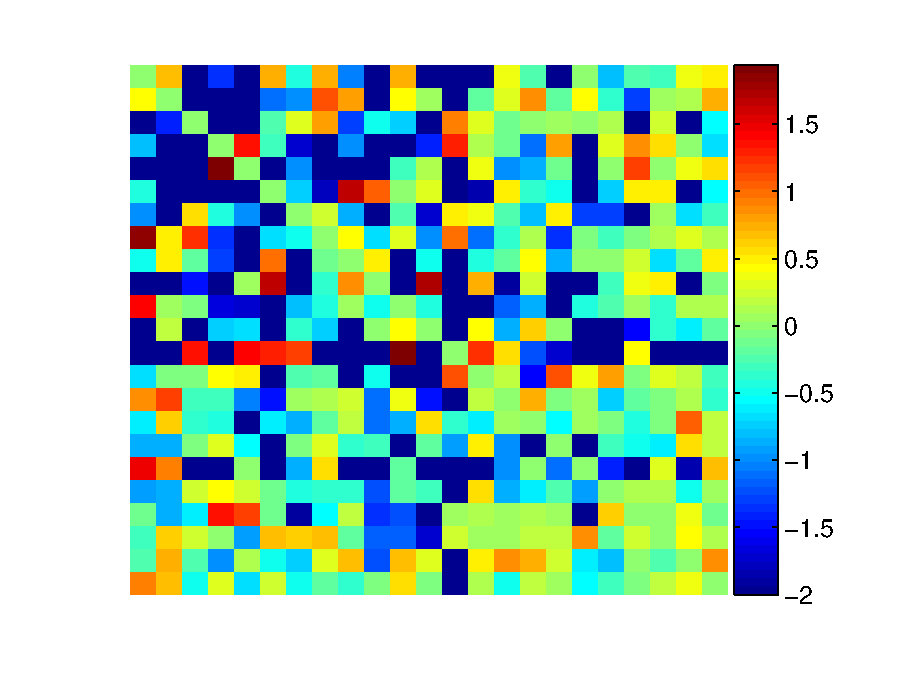
\includegraphics[width=\hsize]{../figs/FigureA11_real_glm}
% \end{minipage}
% \begin{minipage}[c]{0.3\hsize}
% 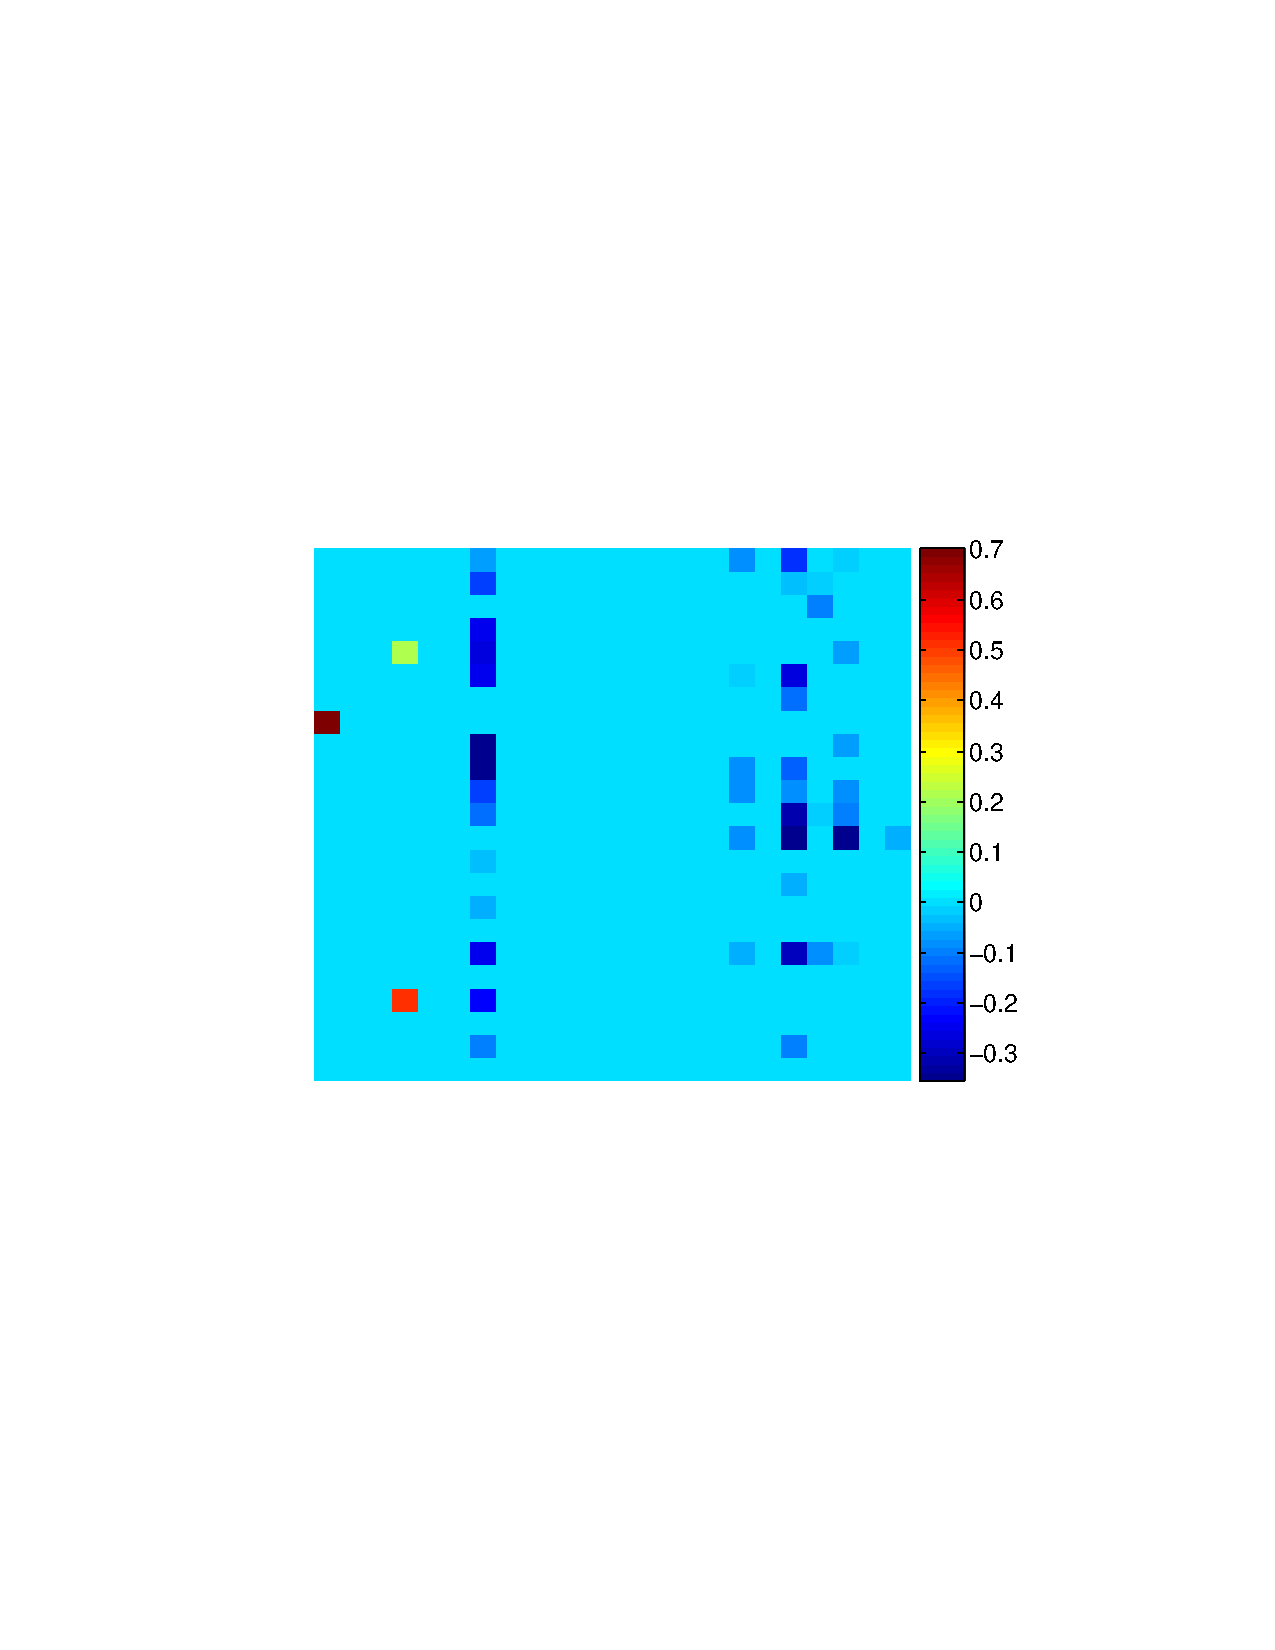
\includegraphics[width=\hsize]{../figs/FigureA11_real_sparse}
% \end{minipage}
% \caption{Functional connectivity matrix inferred from a sample of actual calcium imaging data for $N=72$ cells in [XXX], imaged for $T\approx 260$ sec at 15 Hz.
% $N=23$ neurons with spikes at sufficient SNR were selected, and functional connectivity reconstructed using factorized approximation algorithm. Firing cell of these cells was 0.1-1 Hz and 20-200 spikes were collected for each neuron.
% Upper-left panel shows example of actual fluorescence traces from selected cells, best to worst. Upper-right panel shows a raster of inferred spike trains for first 100 sec of imaging data. Lower panels show left-to-right the time-delayed cross-correlation matrix for selected neurons, simple GLM solution and sparse GLM solution, respectively. A consistent connectivity matrix is obtained here, with sparse solution having sparseness of $\approx 10 \%$, and all neurons automatically respecting Dale's law without explicitly enforcing it. Two clearly excitatory, and three clearly inhibitory neurons can be seen, with remaining neurons not showing significant couplings.}
% \label{fig:real}
% \end{figure}

%We applied our algorithm to a sample of the real calcium imaging data from [XXX], totaling about 5 minutes of imaging for a population of 72 cells in [XXX]. Out of these, about 23 cells had fluorescence traces indicative of spikes, while the other cells were either silent or did not shown SNR sufficient for analysis. These 23 cells were selected for futher processing. 20-200 spikes were found for each cell, corresponding to firing rates from 0.07 Hz to 0.8 Hz.
%We then identified functional connectivity matrix for this population. Sparse solution resulted in consistent connectivity matrix with sparseness of about 10\%, automatically respecting Dale's law, and clearly indicating two strongly connected excitatory neurons and few inihibitory neurons. Although this data lacked independent controls necessary to properly evaluate quality of our obtained reconstruction, it does demonstrate that our approach can be successfully applied under real-life condition to analyze functional connectivity of real populations of neurons.
